\section{使字典攻击更难实施}

当在服务器上存储弱口令的哈希时,离线字典攻击,尤其是基于预处理的离线字典攻击是一种真正的威胁。本节中,我们将讨论一些针对性的技术,这些技术能够使得字典攻击更加困难。

\subsection{公共盐}

上一节中,我们展示了攻击者如何对字典 $\mathcal{D}$ 进行预处理以构建一个速查表 $L$,进而可以快速破解一个或多个哈希后的口令。一种叫做\textbf{加盐(salting)}的简单防御措施就可以反制这种预处理攻击。就算允许攻击者拥有无限时间对 $\mathcal{D}$ 进行预处理,加盐也可以将破解一个哈希口令文件 $F$ 的时间复杂度提升到:
$$
\Omega(|\mathcal{D}|\times |F|)
$$
换言之,加盐可以确保没有任何其他方法的效率优于基于穷举搜索的暴力破解。

加盐的具体做法是在注册新口令时生成一个称为\textbf{盐(salt)}的随机字符串。系统中的每个用户都会被分配一个新的盐,我们可以认为盐是从一个集合 $\mathcal{S}$ 中随机选出的。在实践中,往往 $|\mathcal{S}|=2^{128}$ 就足以满足要求。这个盐会与口令一起被哈希,得到验证密钥 $vk$。盐也会被存储在服务器的口令表中,如图 \ref{fig:18-4} 所示。只有服务器需要知道盐值,用户甚至不需要知道有盐的存在。

\begin{figure}
  \centering
  

\tikzset{every picture/.style={line width=0.75pt}} %set default line width to 0.75pt        

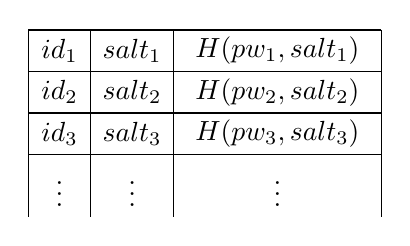
\begin{tikzpicture}[x=0.75pt,y=0.75pt,yscale=-1,xscale=1]
%uncomment if require: \path (0,94); %set diagram left start at 0, and has height of 94

%Straight Lines [id:da48690891710689943] 
\draw  [line width=0.5]  (0,0) -- (0,90) ;
%Straight Lines [id:da07883832722873985] 
\draw  [line width=0.5]  (0,0) -- (170,0) ;
%Straight Lines [id:da39136603292686534] 
\draw  [line width=0.5]  (30,0) -- (30,90) ;
%Straight Lines [id:da18677337990047116] 
\draw  [line width=0.5]  (170,0) -- (170,90) ;
%Straight Lines [id:da7111238231534653] 
\draw  [line width=0.5]  (0,20) -- (170,20) ;
%Straight Lines [id:da28765771561296405] 
\draw  [line width=0.5]  (0,40) -- (170,40) ;
%Straight Lines [id:da41036851267981467] 
\draw  [line width=0.5]  (0,60) -- (170,60) ;
%Straight Lines [id:da9078156775792283] 
\draw  [line width=0.5]  (70,0) -- (70,90) ;

% Text Node
\draw (15,10) node    {$id_{1}$};
% Text Node
\draw (15,30) node    {$id_{2}$};
% Text Node
\draw (15,50) node    {$id_{3}$};
% Text Node
\draw (15,75) node    {$\vdots $};
% Text Node
\draw (120,10) node    {$H( pw_{1} ,salt_{1})$};
% Text Node
\draw (50,75) node    {$\vdots $};
% Text Node
\draw (50,10) node    {$salt_{1}$};
% Text Node
\draw (50,30) node    {$salt_{2}$};
% Text Node
\draw (50,50) node    {$salt_{3}$};
% Text Node
\draw (120,30) node    {$H( pw_{2} ,salt_{2})$};
% Text Node
\draw (120,50) node    {$H( pw_{3} ,salt_{3})$};
% Text Node
\draw (120,75) node    {$\vdots $};


\end{tikzpicture}
  \caption{口令文件(版本2)}
  \label{fig:18-4}
\end{figure}

于是我们就有了新的口令协议,我们称之为\textbf{口令协议版本2},它的运行方式如下:
\begin{itemize}
	\item $G$:令 $pw \xleftarrow{\rm R}\mathcal{P}$,$salt\overset{\rm R}\leftarrow\mathcal{S}$,计算 $y\leftarrow H(pw,salt)$,输出 $sk=pw$ 和 $vk=(salt,y)$。
	\item 以 $sk=pw$ 为输入的算法 $P$ 和以 $vk=(salt,y)$ 为输入的算法 $V$,按如下逻辑交互:
	\begin{enumerate}
		\item $P$ 将 $pw$ 发送给 $V$;
		\item 如果收到的 $pw$ 满足 $H(pw,salt)=y$,$V$ 输出 $\mathsf{accept}$,否则输出 $\mathsf{reject}$。
	\end{enumerate}
\end{itemize}
与版本 1 的描述一样,版本 2 的描述也是相当理想化的,因为我们假设口令 $pw$ 是从空间 $\mathcal{P}$ 中随机均匀选出的,但实际情况远非如此。

现在有了盐的存在,对手可以采取两种策略去攻击文件 $F$ 中的哈希口令:

\begin{itemize}
	\item 第一种策略是使用批量离线字典攻击。问题是,现在预处理阶段需要考虑哈希函数 $H$ 的庞大的输入集合,事实上集合 $\mathcal{D}\times\mathcal{S}$ 中的任何元素都是可能的输入。因此,如果仍然采用式 \ref{eq:18-2} 中的预处理算法,需要准备的预处理表 $L$ 的规模将达到 $|\mathcal{D}|\times|\mathcal{S}|$。这个大小无论如何都是难以生成的,更不要说出村了。因此,式 \ref{eq:18-2} 所介绍的预处理方法不再可行。
	\item 第二种策略是对 $F$ 中的所有口令进行穷举搜索,就像式 \ref{eq:18-1} 中所做的那样。我们已经说明过,穷举搜索的时间复杂度是
	$$O(|\mathcal{D}|\times |F|)$$
\end{itemize}

为了使得没有任何其他方法的效率优于穷举搜索,即上面的第二种策略,盐值空间 $\mathcal{S}$ 需要尽可能大。即使对手采用时空权衡的方法来对$\mathcal{D}\times\mathcal{S}$进行预处理,也同样应该成立。为了推导对 $\mathcal{S}$ 大小的必要约束,我们首先需要更精确地定义在预处理模型中逆转加盐函数的含义。

\begin{snote}[带有预处理的加盐单向函数.]
为了便于定义,我们将对手 $\mathcal{A}$ 拆分成两个独立的对手 $\mathcal{A}_0$ 和 $\mathcal{A}_1$,其中对手 $\mathcal{A}_0$ 拥有无限运行时间,执行预处理阶段。对手 $\mathcal{A}_1$ 能够高效地进行反转攻击。两个对手之间唯一允许的通信是交换一个 $\ell$ 比特的字符串 $L$,其中 $L$ 是预处理阶段的结果。这些概念在下面的定义中得到了体现,该定义将$H$建模为一个随机预言机。
\end{snote}

\begin{definition}\label{def:18-3}
	假设 $H$ 是一个定义在 $(\mathcal{D}\times\mathcal{S},\mathcal{Y})$ 上的哈希函数。我们定义对手 $\mathcal{A}=(\mathcal{A}_0,\mathcal{A}_1)$ 在预处理模型中攻破哈希函数 $H$ 的单向性的优势为 ${\rm OWsp^{ro}\mathsf{adv}}[\mathcal{A},H]$,其大小为对手 $\mathcal{A}$ 赢得下面游戏的概率:
	\begin{itemize}
		\item $\mathcal{A}_0$ 向 $H$ 发起查询并输出一个建议字符串 $L$;
		\item 挑战者随机选择 $(pw,s)\overset{\rm R}\leftarrow\mathcal{D}\times\mathcal{S}$,令 $y=H(pw,s)$,并将 $(L,y,s)$ 发送给 $\mathcal{A}_1$;
		\item $\mathcal{A}_1$ 向 $H$ 发起查询并输出 $pw'\in\mathcal{D}$。当 $H(pw',s)=y$ 时,$\mathcal{A}$ 获胜。
	\end{itemize}
\end{definition}

需要注意的是,对手 $\mathcal{A}_1$ 同时获得了 $L$ 和盐 $s$,而它的目的是找到带有盐 $s$ 的哈希 $y$ 的原象。下面的定理给出了在预处理模型中反转加盐单向函数 $H$ 的时间界限,其中 $H$ 符合随机预言机模型。

\begin{theorem}\label{theo:18-2}
	假设 $H$ 是一个定义在 $(\mathcal{D}\times\mathcal{S},\mathcal{Y})$ 上的哈希函数,$H$ 符合随机预言机模型,且 $|\mathcal{D}|\leq|\mathcal{Y}|$。令 $\mathcal{A}=(\mathcal{A}_0,\mathcal{A}_1)$ 是一个定义 \ref{def:18-3} 中的对手,其中 $\mathcal{A}_0$ 输出一个 $\ell$ 比特的建议字符串 $L$,$\mathcal{A}_1$ 最多能向 $H$ 发起 $Q_{\rm ro}$ 次查询,则有:
	\begin{equation}
	{\rm OWsp^{ro}\mathsf{adv}}[\mathcal{A},H]
	\leq
	O\left(\frac{\ell\cdot Q_{\rm ro}}{|\mathcal{S}|\cdot |\mathcal{D}|}+\frac{Q_{\rm ro}}{|\mathcal{D}|}\right)	
	\end{equation}
\end{theorem}

该定理表明,如果 $\mathcal{A}$ 在反转 $vk:=y\in\mathcal{Y}$ 时有恒定成功概率,比如 $0.5$,那么它在攻击阶段必须至少花费 $Q_{\rm ro}\geq\Omega({|\mathcal{D}|\cdot|\mathcal{S}|}/{\ell})$ 的时长。因此,为了防止预处理带来的破解性能提升,我们应该令 $|\mathcal{S}|\geq\Omega(\ell)$,这会确保不会有其他方法效率优于穷举搜索。比如说,如果我们假设建议字符串 $L$ 的最大存储空间为 $2^{80}$,那么盐空间应当至少是 $\{0,1\}^{80}$。在实践中,人们通常取 $|\mathcal{S}|:=\{0,1\}^{128}$。

从技术上讲,定理 \ref{theo:18-2} 限定了破解\emph{单个}口令的时间,但并没有限定\emph{批量}离线字典攻击的时间。在这种情况下,攻击者可以尝试一次性破解 $t$ 个口令,其中$t>1$。然而,我们希望该定理可以被推广到批量攻击中,使得约束 $|\mathcal{S}|\geq\Omega(\ell)$ 即使面对批处理场景仍能够有效防止破解。

\begin{snote}[加盐的局限性.]
虽然加盐可以抵御预处理攻击,但它并不能阻止其他攻击。比如说,即使使用了盐,一个选择了弱口令的用户仍然容易受到式 \ref{eq:18-1}  中的那种离线字典攻击。在接下来的内容中,我们将展示如何对离线字典攻击提供进一步的保护。
\end{snote}

\subsection{秘密盐}

通过向人类口令中添加人工熵,我们可以使对手的破解变得更难。想法是从一个小空间 $\mathcal{S}_{\rm p}$ 中再随机挑选一个短字符串,称为\textbf{秘密盐 (secret salt)}或者\textbf{胡椒 (pepper)},并将其也纳入到哈希计算中。但是秘密盐\emph{不会}被记录在口令文件中,因此产生的口令文件如图 \ref{fig:18-5} 所示。

\begin{figure}
  \centering
  

\tikzset{every picture/.style={line width=0.75pt}} %set default line width to 0.75pt        

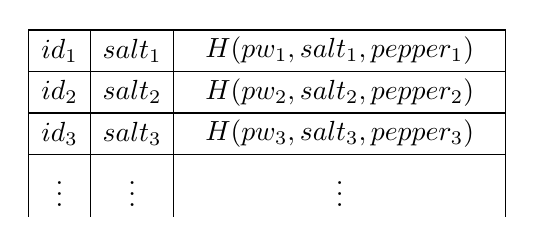
\begin{tikzpicture}[x=0.75pt,y=0.75pt,yscale=-1,xscale=1]
%uncomment if require: \path (0,94); %set diagram left start at 0, and has height of 94

%Straight Lines [id:da26114694722535137] 
\draw  [line width=0.5]  (0,0) -- (0,90) ;
%Straight Lines [id:da05297602560894288] 
\draw  [line width=0.5]  (0,0) -- (230,0) ;
%Straight Lines [id:da6769376854040197] 
\draw  [line width=0.5]  (30,0) -- (30,90) ;
%Straight Lines [id:da014741377443619808] 
\draw  [line width=0.5]  (230,0) -- (230,90) ;
%Straight Lines [id:da7062699917070598] 
\draw  [line width=0.5]  (0,20) -- (230,20) ;
%Straight Lines [id:da9213052228205383] 
\draw  [line width=0.5]  (0,40) -- (230,40) ;
%Straight Lines [id:da18806343487898314] 
\draw  [line width=0.5]  (0,60) -- (230,60) ;
%Straight Lines [id:da529477996966244] 
\draw  [line width=0.5]  (70,0) -- (70,90) ;

% Text Node
\draw (15,10) node    {$id_{1}$};
% Text Node
\draw (15,30) node    {$id_{2}$};
% Text Node
\draw (15,50) node    {$id_{3}$};
% Text Node
\draw (15,75) node    {$\vdots $};
% Text Node
\draw (150,10) node    {$H( pw_{1} ,salt_{1} ,pepper_{1})$};
% Text Node
\draw (50,75) node    {$\vdots $};
% Text Node
\draw (50,10) node    {$salt_{1}$};
% Text Node
\draw (50,30) node    {$salt_{2}$};
% Text Node
\draw (50,50) node    {$salt_{3}$};
% Text Node
\draw (150,30) node    {$H( pw_{2} ,salt_{2} ,pepper_{2})$};
% Text Node
\draw (150,50) node    {$H( pw_{3} ,salt_{3} ,pepper_{3})$};
% Text Node
\draw (150,75) node    {$\vdots $};


\end{tikzpicture}
  \caption{口令文件(版本3)}
  \label{fig:18-5}
\end{figure}

为了验证一个口令,服务器只需要遍历秘密盐的所有可能值,直至找到一个能与存储的哈希值匹配的值。依此设计的\textbf{口令协议(版本 3)}按如下方式运行:
\begin{itemize}
	\item $G$:令 $pw\overset{\rm R}\leftarrow\mathcal{P}$,$salt\overset{\rm R}\leftarrow\mathcal{S}$,$pepper\overset{\rm R}\leftarrow\mathcal{S}_p$,$y\leftarrow H(pw,salt,pepper)$,输出 $sk:=pw$ 和 $vk:=(salt,y)$。
	\item 以 $sk=pw$ 为输入的算法 $P$ 及以 $vk=(salt,y)$ 为输入的算法 $V$,按如下逻辑交互:
	\begin{enumerate}
		\item $P$ 将 $pw$ 发送给 $V$;
		\item 对于收到的 $pw$,如果存在 $p\in\mathcal{S}_{\rm p}$ 满足 $H(pw,salt,p)=y$,$V$ 输出 $\mathsf{accept}$,否则输出 $\mathsf{reject}$。
	\end{enumerate}
\end{itemize}

一个典型的设计是将秘密盐空间设置为 $\mathcal{S}_{\rm p}:=\{0,1\}^{12}$。与版本 2 协议相比,这会使得服务器上的口令验证时长变为原来的 $4096$ 倍,但这在现代计算机上仍然只需要不到百分之一秒的时间,因此用户无法察觉到。然而更重要的是,对手现在破解口令文件中的弱口令的难度也增长到了原来的 $4096$ 倍。

秘密盐使离线字典攻击更加困难,因为现在对手必须在 $\mathcal{D}×\mathcal{S}_{\rm p}$ 空间中搜索,而不仅仅是 $\mathcal{D}$。这种技术对用户体验的影响很小。秘密盐增加了用户口令的熵,但并没有迫使用户记住更复杂的口令。

\subsection{慢哈希函数}

保护弱口令的另一种方法是使用慢哈希函数。回顾一下,用 SHA256 这样的哈希函数对口令进行哈希是非常快的,因此 SHA256 也使得离线字典攻击可能发动成功。现在假设服务器使用一个更慢的哈希函数对口令进行哈希,比如该函数处理一个输入需要百分之一秒,这比 SHA256 慢一万倍左右。尽管这对用户体验的影响微乎其微,但是对手这时再想要对字典中的所有项进行哈希的工作量就增大了一万倍。

那么我们如何构造一个慢哈希函数呢?一个直观的方法就是把一个快速哈希函数迭代足够多的次数,直至它变得很慢。具体地,对于一个定义在 $(\mathcal{X},\mathcal{X})$ 上的哈希函数 $H$,我们现在定义:
\begin{equation}\label{eq:18-5}
	H^{(d)}(x)=H(H(H(\cdots(x)\cdots)))
\end{equation}
这样就将 $H$ 迭代了 $d$ 次,可参见第 14.3 节。如果 $d=10000$,那么计算 $H^{(d)}(x)$ 就比计算 $H(x)$ 要多花一万倍的时间。然而这种方法是有问题的,它也不应该被应用到现实的系统中去。原因之一是,函数 $H^{(d)}(x)$ 也比函数 $H(x)$ 容易逆运算 $d$ 倍,参见练习 14.17。我们下面会介绍一个性质更好的函数。首先,我们先对慢哈希函数进行严格的定义。

\begin{definition}
	一个\textbf{基于口令的密钥推导函数(password-based key derivation function, PBKDF)}是这样的一个函数 $H$,其输入是一个口令 $pw\in\mathcal{P}$,一个空间 $\mathcal{S}$ 中的盐,以及一个难度参数 $d\in\mathbb{Z}^{>0}$;其输出是一个值 $y\in\mathcal{Y}$。我们要求函数 $H$ 能由一个运行时间与 $d$ 成正比的算法有效计算。像往常一样,我们称 PBKDF 定义在 $(\mathcal{P},\mathcal{S},\mathcal{Y})$ 上。
\end{definition}

我们会在练习 18.3 中讨论 PBKDF 的安全要求。我们的第一个 PBKDF 的例子,不妨称之为 \textbf{PBKDF1},就基于式 \ref{eq:18-5},其定义为:
$$
{\rm PBKDF1}_H(pw,salt,d)=H^{(d)}(pw,salt)
$$
对于定义在 $(\mathcal{X},\mathcal{X})$ 上的哈希函数 $H$,PBKDF1 定义在 $(\mathcal{P},\mathcal{S},\mathcal{X})$ 上,其中 $\mathcal{X}=\mathcal{P}\times\mathcal{S}$。由于存在练习 14.17 中所介绍的攻击方式,该构造不会被应用在实际的系统中。

\subsubsection{PBKDF2 函数}

一种在实践中被广泛用于构造慢哈希函数的方法被称为PBKDF2。令 $F$ 是一个定义在 $(\mathcal{P},\mathcal{X},\mathcal{X})$ 上的PRF,其中 $\mathcal{X}:=\{0,1\}^n$,那么由之派生出的 PBKDF,不妨用 $\text{PBKDF2}_F$ 表示,它也定义在$(\mathcal{P},\mathcal{X},\mathcal{X})$ 上,并按如下方式工作:
\begin{equation}\label{eq:18-6}
	{\rm PBKDF2}_F(pw,salt,d):=
	\left\{
	\begin{aligned}
		& x_0\leftarrow F(pw, salt)\\
		& \text{for }i=1,\dots,d-1:\\
		& ~~~~~~x_i\leftarrow F(pw,x_{i-1})\\
		& \text{output }y\leftarrow x_0 \oplus x_1 \oplus \cdots \oplus x_{d-1}\in\mathcal{X}
	\end{aligned}
	\right\}
\end{equation}
上面的式 \ref{eq:18-6} 描述了基本版的 PBKDF2,如果需要输出更多比特,对其稍加调整即可。事实上,PBKDF2 能够输出 $\mathcal{X}^b$ 中的一个元素,其中 $1<b<2^{32}$,方法是计算:
\begin{equation}\label{eq:18-7}
{\rm PBKDF2}_F^{(b)}(pw,salt,d):=
\left(
{\rm PBKDF2}_F(pw,salt_1,d),\dots,
{\rm PBKDF2}_F(pw,salt_b,d)
\right)
\in\mathcal{X}^b
\end{equation}
其中所有的$b$个盐都是由最初给定的盐派生而来的,方法是令$salt_i\leftarrow salt\,||\,{\rm bin}(i)$。这里的${\rm bin}(i)$是$i\in\{1,\dots,b\}$的32位二进制字符串表示。

在实践中,PBKDF2 通常使用 HMAC-SHA256 作为底层 PRF。难度 $d$ 的设置取决于项目需求和硬件速度。例如,iOS 10 中的备份钥匙包使用 PBKDF2 来保护,其中 $d$ 的值是一千万。在Windows 10 中,数据保护 API 默认使用 $d = 8000$,但使用 HMAC-SHA512 作为 PRF。

我们会在练习18.2和18.3中更详细地讨论PBKDF2的安全性。

\subsection{慢内存困难哈希函数}

PBKDF2 的一个重要问题是它容易受到并行硬件攻击。我们知道,大部分现代处理器都是基于缓存的,而计算单元只占整个处理器面积的一小部分。因此,一个商用处理器不能对许多输入进行并行 PBKDF2 计算,也不太适合进行离线字典攻击。

更有经验的攻击者通常会在支持高度并行的专用硬件上运行离线字典攻击,比如 GPU,FPGA,甚至是定制芯片。一个定制芯片可以包装超过一百万个 SHA256 计算单元。如果每个单元每秒可以进行一百万次 SHA256 计算,那么一个对手每秒可以在每个芯片上尝试 $10^{12}$ 个口令。即使 PBKDF2 的难度被设置为 $d=10000$,一个由大约 500 个这样的专用芯片组成的农场也能在不到一天的时间内跑完所有 $2^{52}$ 个 8 位口令。这种攻击之所以能够实现,是因为 SHA256 的硬件实现可以做得相当紧凑,所以大量的 SHA256 计算单元可以打包到一个芯片里。

这表明,我们需要的哈希函数 $H$ 应该要求专用硬件实现也需要庞大的片上面积,这样一个芯片就只能容纳几个计算单元,这就极大程度上降低了定制硬件的性能优势。

那么我们如何建立一个具有较大硬件占用面积的哈希函数 $H$?一种方法是确保计算 $H$ 的每一步都需要大量的内存,这将迫使攻击者将芯片上的大部分区域分配给单次哈希求值所需的内存,这就确保了每个芯片只能包含少量的计算电路。

需要大量内存的哈希函数被称为\textbf{内存困难函数}。已经有一些符合要求的内存难度哈希函数,这些函数能够在随机预言机模型下被严格证明是内存困难的。在我们讨论安全问题之前,让我们先看看一个流行的结构,叫做\textbf{Scrypt}。Scrypt是由一个内存容易的哈希函数$h:\mathcal{X}\rightarrow\mathcal{X}$,其中$\mathcal{X}:=\{0,1\}^n$。得到的函数记作$\text{Scrypt}_h$,如图 \ref{fig:18-6} 所示。

\begin{figure}
    \hspace*{5pt} 输入:$x_0\in\mathcal{X}$,难度 $d\in\mathbb{Z}^{>0}$

	\vspace{3pt}

	\hspace*{5pt} 1.
	\hspace*{20pt} 对于 $i=1,\dots,d$: 令 $x_i\leftarrow h(x_{i-1})$
	\hspace*{20pt} //\quad\emph{那么}$x_i=h^{(i)}(x_0)$\\
	\hspace*{5pt} 2.
	\hspace*{20pt} 令 $y_0\leftarrow x_d$\\
	\hspace*{5pt} 3.
	\hspace*{20pt} 对于 $i=1,\dots,d$:\\
	\hspace*{5pt} 4.
	\hspace*{50pt} 令 $j\leftarrow\mathrm{int}(y_{i-1})\bmod(d+1)$
	\hspace*{16pt} //\quad$\mathrm{int}(y_{i-1})$\emph{将}$y_{i-1}\in\mathcal{X}$\emph{转换为一个整数}\\
	\hspace*{5pt} 5.
	\hspace*{50pt} 令 $y_i\leftarrow h(y_{i-1}\oplus x_j)$
	\hspace*{52pt} //\quad\emph{从数组}$(x_0,\dots,x_d)$\emph{中读取一个随机位置}
	
	\vspace{3pt}
	
	\hspace*{5pt} 输出 $y_d\in\mathcal{X}$
	\caption{函数$\mathrm{Scrypt}_h(x_0,d)$}
  \label{fig:18-6}
\end{figure}

在我们的安全分析中,我们将底层哈希函数 $h$ 当作一个随机预言机。在实践中,函数 $h$ 是由 Salsa 20/8 变换衍生出来的,参见3.6节。难度 $d$ 是根据系统的性能需求来设置的。例如我们可以设置一个恰当的 $d$ 使得计算 Scrypt 需要填满整个芯片的存储空间。这会确保计算 Scrypt 不会太慢,但需要大量的内存。

图 \ref{fig:18-6} 是将Scrypt作为一个哈希函数的描述。另一方面,定义在 $(\mathcal{P},\mathcal{X},\mathcal{X})$ 上的Scrypt PBKDF是基于Scrypt哈希构建的,其工作原理如下:
\begin{equation}\label{eq:18-8}
	{\rm ScryptPBKDF}_h(pw,salt,d):=
	\left\{
	\begin{aligned}
		& x_0\leftarrow {\rm PBKDF2}_F(pw,salt,1)\\
		& y\leftarrow \text{Scrypt}_h(x_0,d)\\
		& \text{output }{\rm PBKDF2}_F(pw,y,1)
	\end{aligned}
	\right\}
\end{equation}
其中 $F$ 是一个定义在 $(\mathcal{P},\mathcal{X},\mathcal{X})$ 上的 PRF。在实践中,我们通常使用HMAC-SHA256作为$F$。如有需要,我们也可多次迭代 Scrypt,以使其速度更慢而不增加所需的内存。同样地,通过调整最后一行的PBKDF2的应用,它可以在$b>1$时输出$\mathcal{X}^b$中的一个元素,就像式 \ref{eq:18-7} 那样。

\begin{snote}[Scrypt 是内存困难的吗?]
通过存储 $\mathcal{X}$ 中的 $d+1$ 个元素,Scrypt 函数可以在 $O(d)$ 时间内被计算。Scrypt 哈希的构建步骤创建了一个大小为 $d+1$ 的数组 $(x_0,\dots,x_d)$,随后重复地从该数组中的随机位置读取数据。正因此,一个想要在 $O(d)$ 时间内完成计算的算法必须在内存中保存整个数组 $(x_0,\dots,x_d)$。但这个结论尚需严格证明。

危险的是,时空权衡可能使攻击者尝试牺牲更多的攻击时间来换取更少的内存消耗。这将是毁灭性的,因为减少的内存将允许攻击者将许多 Scrypt 计算单元打包到一个芯片中,而这正是我们想要极力避免的。

在练习18.6中,我们设计了一种针对Scrypt的简单的时空权衡。它表明对于任意的$1<\alpha<d/2$,只需要存储$\lceil d/\alpha\rceil$ 个$\mathcal{X}$中的元素,就可以在$O(\alpha d)$的时间内完成对 Scrypt 的计算。特别地,使用\emph{恒定}空间的Scrypt可以在$O(d^2)$时间内完成计算。然而这种类型的时空权衡并不能帮助对手。对手需要将$\alpha$倍的Scrypt计算单元装入一个芯片中,但每个计算单元的工作难度也变为原来的$\alpha$倍。因此与图 \ref{fig:18-6} 中的Scrypt实现相比,单个芯片的整体吞吐量并没有变化。尽管如此,我们仍然需要证明没有比Scrypt更好的时空权衡方案。

流水线是对内存难度的另一个威胁。假设存在一个算法,它在计算 Scrypt 时仅仅在算法的其中几个步骤中需要使用 $O(d)$ 的内存。如果算法在其余步骤中仅需要使用常数级的内存空间,那么攻击者就可以通过构建流水线来排列多个 Scrypt 计算单元,这些计算单元之间共享一个 $O(d)$ 大小的存储。这样,每个计算单元仅在它需要 $O(d)$ 存储的几个步骤中调用内存,在其他时间可以把存储释放给其他计算单元使用。这样一来,攻击者仍然可以把许多计算单元打包到一个芯片中,只需要共享一个 $O(d)$ 大小的存储阵列即可。为了防止这种形式的流水线,我们还需要证明每一个 Scrypt 实现都需要\emph{在许多计算步骤中}使用到 $O(d)$ 级别的内存。
\end{snote}

\begin{snote}[Scrypt 是内存困难的.]
为了证明 Scrypt 是内存困难的,我们首先需要定义一个安全模型来分析上面讨论的几种障碍。我们下面定义了一个抽象的并行随机预言机模型,其中的算法 $\mathcal{A}$ 能够并行查询多个输入在随机预言机 $h:\mathcal{Y}\to\mathcal{Z}$ 上的输出。

一个\textbf{并行随机预言机算法} $\mathcal{A}$ 将一个 $x\in\mathcal{X}$ 作为输入,并进行一系列的状态转换。在每个状态下,算法 $\mathcal{A}$ 都会向随机预言机 $h$ 发出一组查询,算法在收到查询的所有响应后就会转入下一状态。该过程将不断重复,直至算法终止,此时算法到达最终状态,其中包含算法的输出。所有中间状态都需要被记录,以便跟踪中间状态的大小。

形式上说,算法 $\mathcal{A}$ 实现了一个确定性映射:
$$\mathcal{A}:\mathcal{X}\times\mathcal{S}\times\mathcal{Z}^{\leq p}\to\mathcal{S}\times\mathcal{Y}^{\leq p}$$
其中 $p$ 是正整数,其工作流程如下:
\begin{itemize}
	\item $\mathcal{A}$ 被作为 $\mathcal{A}(x,\varepsilon,\varepsilon)$ 调用,它输出一个 $\mathcal{S}\times\mathcal{Y}^{\leq p}$ 中的元组 $(s_1,\overline y_1)$。这里,$s_1$ 是 $\mathcal{A}$ 的当前状态,$\overline y_1=(y_1,\dots,y_r)$ 是它对随机预言机 $h:\mathcal{Y}\to\mathcal{Z}$ 所发出的第一组并行查询。
	\item 对于 $i=1,\dots,t$,当 $\mathcal{A}$ 输出 $(s_i,\overline y_i)$,$\overline y_1=(y_1,\dots,y_r)\in\mathcal{Y}^{\leq p}$ 时,我们进行如下操作:
	\begin{itemize}
	  \item 并行地调用随机预言机 $h$,计算$\overline z_i\leftarrow (h(y_1),\dots,h(y_r))$,并且
	  \item 重新调用 $\mathcal{A}$ 并计算 $(s_{i+1},\overline y_{i+1})\leftarrow \mathcal{A}(x,s_i,\overline z_i)$。
	\end{itemize}
	\item 最终 $\mathcal{A}$ 输出 $(s,\varepsilon)$,这表示算法终止,输出值为 $s$。
\end{itemize}

算法 $\mathcal{A}$ 在输入 $x\in\mathcal{X}$ 上的运行时间就是 $\mathcal{A}$ 在终止之前被调用的总次数。以这种方式衡量运行时间,我们可以捕捉到一个事实,即硬件实现可以在多点上并行地计算哈希函数$h$。

我们现在记第 $i$ 步输入 $\mathcal{A}$ 的数据为 $st_i:=(s_i,\overline y_i)$,并称 $st_i$ 为 $i$ 时刻的输入状态。对于 $s\in\mathcal{S}$,我们令 $|s|$ 表示 $s$ 的比特位数,类似地,我们令 $|z|$ 表示 $z\in\mathcal{Z}$ 的长度。对于 $\overline z=(z_1,\dots,z_r)\in\mathcal{Z}^{\leq p}$,我们令 $|\overline z|:=\sum_{j=1}^r|z_i|$。那么当 $\mathcal{Z}=\{0,1\}^n$ 时,我们有 $|\overline z|=rn$。最后,我们将输入状态 $st=(s,\overline z)$ 的长度定义为 $|st|:=|s|+|\overline z|$。
\end{snote}

\begin{definition}
	令 $\mathcal{A}$ 是一个以 $\mathcal{X}$ 中元素作为输入的并行随机预言机算法。记$\mathcal{A}$ 对于随机预言机 $h:\mathcal{Y}\to\mathcal{Z}$ 和 $x\in\mathcal{X}$ 的累计存储复杂度为 ${\rm mem}[\mathcal{A},h,x]$,其定义是:
	$${\rm mem}[\mathcal{A},h,x]:=\sum_{i=1}^t|st_i|$$
\end{definition}

图 \ref{fig:18-6} 中对于预言机$h:\mathcal{X}\to\mathcal{X}$,$\mathcal{X}=\{0,1\}^n$计算$\text{Scrypt}_h(x,d)$的算法的累计存储复杂度是$O(nd^2)$。下面的定理将表示,这种设计是最优的。

\begin{theorem}\label{theo:18-3}
	令 $\mathcal{X}=\{0,1\}^n$ 是一个满足 $|\mathcal{X}|$ 为超多项式的空间,$d$ 为一个使得 $2^{-d}$ 可以忽略不计的值。对于所有的并行随机预言机算法 $\mathcal{A}$ 和所有的 $x\in\mathcal{X}$,都有:
	$$
	  {\rm Pr}
	  \left[
	    \mathcal{A}(x,d)={\rm Scrypt}_h(x,d)
	  \right]
      \leq
      {\rm Pr}
      \left[
      {\rm mem}[\mathcal{A},h,(x,d)]\geq\Omega(d^2n)
      \right]+\delta
    $$
    其中 $\delta$ 是一个可以忽略的值。上面的两个概率都基于随机预言机 $h:\mathcal{X}\to\mathcal{X}$的选择。
\end{theorem}

该定理表明,如果 $\mathcal{A}(x,d)$ 以接近 $1$ 的概率输出 ${\rm Scrypt}_h(x,d)$,那么对于几乎所有的 $h$ 的选择,$\mathcal{A}$ 的累计存储复杂度一定是 $\Omega(d^2n)$ 级的。这表明不可能存在一个针对 Scrypt 的时空权衡策略使得其表现比练习18.6更好。如果一个算法以最大 ${dn}/{\alpha}$ 的存储空间计算 Scrypt,其中 $\alpha>1$,那么它的运行时间必然是 $\Omega(d\alpha)$。否则其累计存储复杂度将突破下限。

同样地,不可能存在对 Scrypt 的流水线式攻击。任何在 $O(d)$ 时间内运行的计算 Scrypt 的可行算法必须在整个算法中使用 $\Omega(d\alpha)$ 的内存。否则其累计存储复杂度也将突破下限。

从技术上讲,定理 \ref{theo:18-3} 限定了在\emph{单一}输入下计算Scrypt所需的时间和空间。它并没有限定\emph{批量}离线字典攻击的时间,此时攻击者试图一次对$p>1$个口令计算Scrypt。然而,我们期望该定理可以被推广到批量的设置中:如果一个算法$\mathcal{A}$对$p$个输入正确地计算了Scrypt的概率接近$1$,那么$\mathcal{A}$的累计存储复杂度一定是$\Omega(d^2np)$。这将表明,在$p$个点上计算Scrypt时,不存在针对Scrypt的时空权衡或流水线攻击。

\subsubsection{模糊口令内存困难函数}

虽然Scrypt是一个健全的内存困难的口令哈希函数,但它很容易受到第4.3.2节中讨论的那种侧信道道攻击。

考虑一个登录服务器,其中一个运行中的进程 $P$ 通过 Scrypt 哈希并验证用户的口令。假设对手获得了对该服务器的低权限访问,对手可以在服务器上运行用户级程序但不能破坏进程 $P$,也不能观察到用户的口令明文。然而,利用这种权限,它仍然可以发起一个名为\textbf{缓存计时攻击 (cache timing attack)} 的巧妙攻击方法,这种攻击能够让攻击者了解到 $P$ 访问内存页的顺序。注意,攻击者并不能知道内存页中存储的内容,它只能获取 $P$ 读取页的顺序。

现在,假设对手捕获了一个哈希值 $y$,它是将式 \ref{eq:18-8} 中介绍的Scrypt PBKDF应用于某个带有公共盐的口令 $pw$ 的结果。通常情况下,对手需要发起一个字典攻击,每次尝试都需要大量的时间和\emph{内存}。然而如果对手掌握了进程 $P$ 在计算$pw$的Scrypt哈希时的的内存访问模式,它就可以用很少的内存对 $pw$ 进行字典攻击。

为了说明如何实现攻击,让我们回顾一下图 \ref{fig:18-6} 中所介绍的Scrypt 的实现。算法在第一次执行第 5 步时,需要从数组$(x_0,\dots,x_d)$读取$j$号元素,其中$j={\rm int}(y_0)\bmod(d+1)$。

通过观察 $P$ 对内存的访问,对手可以看到算法第一次执行第5步时读取了哪一页的内存,这就给了对手一个 $j$ 的近似值 $j_a$。由于一个内存页中可能存储了多个数组单元,所以对手并没有办法获取 $j$ 的精确值。尽管如此,这个 $j_a$ 也足以使用有限的内存来测试一个可能的口令$pw'$,方法是:
\begin{enumerate}
	\item 按式 \ref{eq:18-8} 计算 $x_0'\leftarrow{\rm PBKDF2}_F(pw',salt,1)$,
	\item 如图 \ref{fig:18-6} 那样计算 $y_0'$,但不存储任何中间值,然后
	\item 测试 $j'\leftarrow{\rm int}(y_0')\mod(d+1)$ 是否与 $j_a$ 接近。
\end{enumerate}

如果测试失败,那么 $pw'$ 就不是正确的口令。这个过程让对手用很少的内存就能过滤掉字典中的大部分候选口令。这样,用户的口令又变得容易受到硬件攻击。

\begin{snote}[一个解决方案.]
这种攻击之所以有效,是因为 Scrypt 的内存访问模式取决于用户的口令。如果我们有一个可证明安全的内存困难哈希函数,其内存访问模式与用户的口令无关,那就更好了。它仍然可以依赖于用户的盐,因为盐不是秘密。这样的函数被称为\textbf{数据模糊内存难度函数}。这种函数的一个例子是 \textbf{Argon2i B},它与 Scrypt 密切相关,但其第一部分的内存访问模式与口令无关,这就消解了上面描述的侧信道攻击。
\end{snote}

\begin{snote}[慢哈希与秘密盐.]
总结本小节,我们观察到秘密盐方法和慢哈希方法都会增加对手的工作负荷。人们可以使用其中的一种方法,但不能两者兼用。慢速内存难度哈希方法的主要好处是,它使定制的硬件攻击难以实施。与快速哈希函数一起使用的秘密盐并不能防止并行硬件攻击,因此慢内存困难哈希比秘密盐更可取。
\end{snote}

\subsection{其他口令管理问题}

\begin{snote}[共同口令问题 (common password problem).]
用户经常在多台机器和多个网站上拥有账户。理想情况下,所有这些服务器都会采取适当的预防措施来防止对手获得口令文件,并对口令进行适当的加盐和哈希,以降低对手获得该文件时的损失。不幸的是,低安全性服务器的设计者可能不会采取与高安全性服务器一样的安全预防措施。这种低安全性的服务器可能更容易被入侵。此外,这种低安全性的服务器可能会存储没有盐的口令哈希,这使批量字典攻击成为可能,并将检索出所有的弱口令。更糟糕的是,有些服务器甚至会在明处存储哈希值,这样对手就会检索出所有的口令,甚至是强口令。因此对手可以侵入一个低安全级别的服务器,并在该服务器上检索到一些,甚至所有的用户 ID/口令,而且这些口令中的一些也很有可能被用在高安全级别的服务中。因此,尽管在高安全性的服务器上采取了所有的预防措施,但该服务器的安全性可能会被一些完全不相关的、低安全性的服务器的不良安全性所破坏。这个问题被称为\textbf{共同口令问题}。

解决共同口令问题的一个标准方案是安装客户端软件,它能将通用口令转换为独有的网站口令,也就是个 "客户端盐"。令 $H$ 是一个哈希函数,如果用户名为 $id$ 的用户的口令是 $pw$,这个口令将在登录时发送给服务器 $id_{\rm server}$。用户的客户端或浏览器在发送前会将口令 $pw$ 转换为 $\widehat{pw}:=H(pw,id,id_{\rm server})$,然后将 $\widehat{pw}$ 发送给服务器。这样,从服务器的角度来看,用户的口令是 $\widehat{pw}$,而从用户的角度来看,口令仍然是 $pw$。这种技术可以保证,即使该用户在许多服务器上使用同一个口令,也不会受到那些没有正确加盐和哈希的服务器的影响。
\end{snote}

\begin{snote}[生物识别技术 (biometrics).]
基于口令的认证的最大困难是用户往往会忘记他们的口令。所有支持电话中的很大一部分都与口令相关的问题有关。因此,一些已部署的系统试图用人类生物识别技术来取代口令,如指纹、视网膜扫描、面容识别和许多其他技术。人们甚至可以使用击键动态,即击键之间的时间长度和按下一个键的时长作为一种生物识别特征。这个想法是使用生物特征作为用户的口令。

虽然生物识别技术相比口令而言有明显的好处,例如用户不会忘记他们的指纹,但它有两个明显的缺点:
\begin{itemize}
	\item 生物识别技术通常不是机密的,人们会在他们接触的几乎任何东西上留下他们的指纹;
	\item 生物识别技术是不可逆的,一旦生物识别特征被盗,用户就无法追索。
\end{itemize}
因此,生物识别技术不应该被用作识别用户的唯一手段,只适合作为额外的识别手段(有时被称为第二因素认证)来提高安全性。
\end{snote}